% ============================================================================
% 02_architecture | 04_activation_function
% Section-body file: include immediately after the relevant \section command
% in tstextbook.tex. This file intentionally contains no document class,
% package imports, \chapter, \section, or bibliography command.
% Figures are original TikZ source fragments stored in the root-level
% figures directory. Bibliographic entries are supplied in bibliography.bib.
% ============================================================================

The preceding section established the feed-forward network as the component
that transforms each contextual token representation through learned
projections. Its central operation is a composition of affine mappings with
a nonlinear transformation between them. The mathematical role of that
intermediate transformation is the subject of the present section. An
activation function is not merely a convenient operation inserted between
matrix multiplications: it determines which nonlinear mappings the network
can represent, how derivatives propagate during optimization, and what
numerical and computational costs are incurred. These properties become
particularly consequential in a Transformer, where the same feed-forward
architecture is applied repeatedly across a deep stack of layers
\parencite{han2024review,zhuo2025polycom}.

\subsection{Why nonlinear transformations are indispensable}
\label{subsec:act-nonlinearity}

An affine transformation maps an input vector to an output vector by
multiplying it by a matrix and adding a bias. Under the row-vector convention
used in the preceding feed-forward discussion, let
\(x\in\mathbb{R}^{1\times H}\), let
\(W\in\mathbb{R}^{H\times D}\), and let
\(b\in\mathbb{R}^{1\times D}\). The affine mapping is
\begin{equation}
    z=xW+b,
    \qquad
    z\in\mathbb{R}^{1\times D}.
    \label{eq:act-affine-map}
\end{equation}
The word \emph{affine} is important: when \(b\neq 0\), the mapping is not
linear in the strict algebraic sense, but it is a linear transformation
followed by a translation.

Composing affine transformations does not, by itself, create a nonlinear
function. To see this, consider two successive mappings,
\begin{align}
    z_1 &= xW_1+b_1,
    \label{eq:act-affine-first}
    \\
    z_2 &= z_1W_2+b_2.
    \label{eq:act-affine-second}
\end{align}
Substitution of the first expression into the second gives
\begin{align}
    z_2
    &= (xW_1+b_1)W_2+b_2
    \nonumber\\
    &=x(W_1W_2)+(b_1W_2+b_2).
    \label{eq:act-affine-composition}
\end{align}
Defining
\begin{equation}
    W_{\mathrm{eff}}=W_1W_2,
    \qquad
    b_{\mathrm{eff}}=b_1W_2+b_2,
    \label{eq:act-effective-affine-parameters}
\end{equation}
reduces the composition to
\begin{equation}
    z_2=xW_{\mathrm{eff}}+b_{\mathrm{eff}}.
    \label{eq:act-composed-affine}
\end{equation}
It is therefore still one affine transformation. The same reasoning
extends to any finite sequence of affine layers: without an intervening
nonlinear operation, depth alone does not enlarge the class of functions
beyond affine mappings.

An activation function changes this conclusion. Let
\(\rho:\mathbb{R}\rightarrow\mathbb{R}\) be a scalar nonlinear function.
For a vector input, the standard element-wise convention applies \(\rho\)
to every coordinate independently. A two-projection feed-forward network
can then be written as
\begin{equation}
    \operatorname{FFN}_{\rho}(x)
    =
    \rho(xW_1+b_1)W_2+b_2.
    \label{eq:act-ffn-general}
\end{equation}
Here \(W_1\in\mathbb{R}^{H\times D_{\mathrm{ff}}}\),
\(W_2\in\mathbb{R}^{D_{\mathrm{ff}}\times H}\),
\(b_1\in\mathbb{R}^{1\times D_{\mathrm{ff}}}\), and
\(b_2\in\mathbb{R}^{1\times H}\). The intermediate dimension
\(D_{\mathrm{ff}}\) is the number of features to which the activation is
applied. The bias-free form
\begin{equation}
    \operatorname{FFN}_{\rho}(x)=\rho(xW_1)W_2
    \label{eq:act-ffn-source-form}
\end{equation}
is the formulation used by \textcite{zhuo2025polycom}; the inclusion of
biases does not alter the argument about the need for nonlinearity.

For a complete sequence tensor
\(X\in\mathbb{R}^{B\times S\times H}\), where \(B\) is batch size and
\(S\) is sequence length, the operation acts on the final feature
dimension:
\begin{align}
    Z &= XW_1,
    & Z&\in\mathbb{R}^{B\times S\times D_{\mathrm{ff}}},
    \label{eq:act-batch-projection}\\
    H_{\rho} &= \rho(Z),
    & H_{\rho}&\in\mathbb{R}^{B\times S\times D_{\mathrm{ff}}},
    \label{eq:act-batch-activation}\\
    Y &= H_{\rho}W_2,
    & Y&\in\mathbb{R}^{B\times S\times H}.
    \label{eq:act-batch-output}
\end{align}
The activation changes the feature coordinates of each token representation.
For element-wise functions such as ReLU, GELU, and SiLU, it does not itself
mix different sequence positions. The attention sublayer is responsible for
cross-position information exchange, whereas the feed-forward activation
contributes to the nonlinear transformation of the representation available
at each position \parencite{han2024review,zhuo2025polycom}.

The contrast between an affine composition and a nonlinear feed-forward
mapping is summarized in \cref{fig:act-nonlinearity}. The upper path can be
collapsed into one affine mapping. The lower path cannot generally be
collapsed in this way because the activation intervenes between the two
projections.

\begin{figure}[htbp]
    \centering
    % TikZ source fragment: activation_nonlinearity.tex
% Included by % TikZ source fragment: activation_nonlinearity.tex
% Included by % TikZ source fragment: activation_nonlinearity.tex
% Included by \input{figures/activation_nonlinearity}.
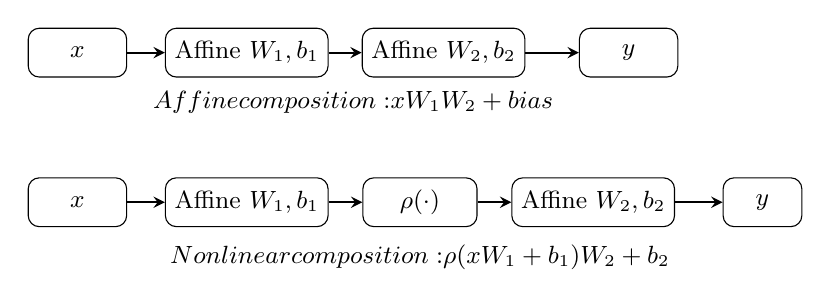
\begin{tikzpicture}[>=stealth, every node/.style={font=\small}]
    \node[draw, rounded corners, minimum width=1.25cm, minimum height=0.62cm]
        (x1) at (0,1.35) {$x$};
    \node[draw, rounded corners, minimum width=1.55cm, minimum height=0.62cm]
        (w11) at (2.15,1.35) {Affine \(W_1,b_1\)};
    \node[draw, rounded corners, minimum width=1.55cm, minimum height=0.62cm]
        (w21) at (4.65,1.35) {Affine \(W_2,b_2\)};
    \node[draw, rounded corners, minimum width=1.25cm, minimum height=0.62cm]
        (y1) at (7.0,1.35) {$y$};
    \draw[->, thick] (x1) -- (w11);
    \draw[->, thick] (w11) -- (w21);
    \draw[->, thick] (w21) -- (y1);
    \node at (3.5,0.72) {\(\text{Affine composition: }xW_1W_2+\text{bias}\)};

    \node[draw, rounded corners, minimum width=1.25cm, minimum height=0.62cm]
        (x2) at (0,-0.55) {$x$};
    \node[draw, rounded corners, minimum width=1.55cm, minimum height=0.62cm]
        (w12) at (2.15,-0.55) {Affine \(W_1,b_1\)};
    \node[draw, rounded corners, minimum width=1.45cm, minimum height=0.62cm]
        (rho) at (4.35,-0.55) {\(\rho(\cdot)\)};
    \node[draw, rounded corners, minimum width=1.55cm, minimum height=0.62cm]
        (w22) at (6.55,-0.55) {Affine \(W_2,b_2\)};
    \node[draw, rounded corners, minimum width=1.0cm, minimum height=0.62cm]
        (y2) at (8.7,-0.55) {$y$};
    \draw[->, thick] (x2) -- (w12);
    \draw[->, thick] (w12) -- (rho);
    \draw[->, thick] (rho) -- (w22);
    \draw[->, thick] (w22) -- (y2);
    \node at (4.35,-1.25)
        {\(\text{Nonlinear composition: }\rho(xW_1+b_1)W_2+b_2\)};
\end{tikzpicture}
.
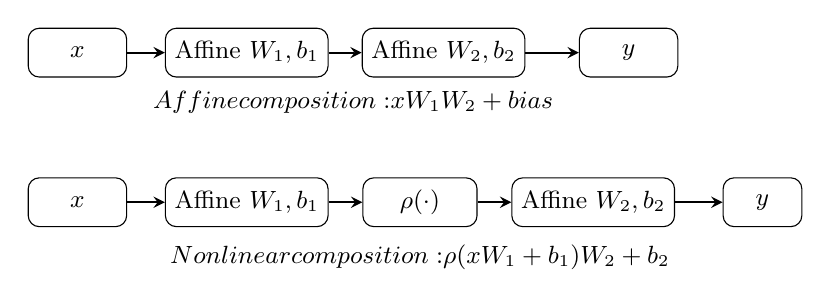
\begin{tikzpicture}[>=stealth, every node/.style={font=\small}]
    \node[draw, rounded corners, minimum width=1.25cm, minimum height=0.62cm]
        (x1) at (0,1.35) {$x$};
    \node[draw, rounded corners, minimum width=1.55cm, minimum height=0.62cm]
        (w11) at (2.15,1.35) {Affine \(W_1,b_1\)};
    \node[draw, rounded corners, minimum width=1.55cm, minimum height=0.62cm]
        (w21) at (4.65,1.35) {Affine \(W_2,b_2\)};
    \node[draw, rounded corners, minimum width=1.25cm, minimum height=0.62cm]
        (y1) at (7.0,1.35) {$y$};
    \draw[->, thick] (x1) -- (w11);
    \draw[->, thick] (w11) -- (w21);
    \draw[->, thick] (w21) -- (y1);
    \node at (3.5,0.72) {\(\text{Affine composition: }xW_1W_2+\text{bias}\)};

    \node[draw, rounded corners, minimum width=1.25cm, minimum height=0.62cm]
        (x2) at (0,-0.55) {$x$};
    \node[draw, rounded corners, minimum width=1.55cm, minimum height=0.62cm]
        (w12) at (2.15,-0.55) {Affine \(W_1,b_1\)};
    \node[draw, rounded corners, minimum width=1.45cm, minimum height=0.62cm]
        (rho) at (4.35,-0.55) {\(\rho(\cdot)\)};
    \node[draw, rounded corners, minimum width=1.55cm, minimum height=0.62cm]
        (w22) at (6.55,-0.55) {Affine \(W_2,b_2\)};
    \node[draw, rounded corners, minimum width=1.0cm, minimum height=0.62cm]
        (y2) at (8.7,-0.55) {$y$};
    \draw[->, thick] (x2) -- (w12);
    \draw[->, thick] (w12) -- (rho);
    \draw[->, thick] (rho) -- (w22);
    \draw[->, thick] (w22) -- (y2);
    \node at (4.35,-1.25)
        {\(\text{Nonlinear composition: }\rho(xW_1+b_1)W_2+b_2\)};
\end{tikzpicture}
.
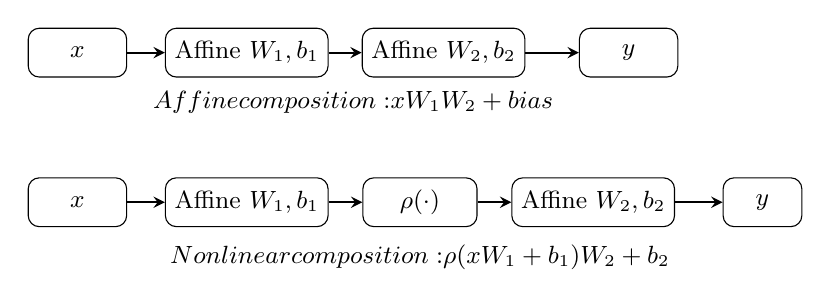
\begin{tikzpicture}[>=stealth, every node/.style={font=\small}]
    \node[draw, rounded corners, minimum width=1.25cm, minimum height=0.62cm]
        (x1) at (0,1.35) {$x$};
    \node[draw, rounded corners, minimum width=1.55cm, minimum height=0.62cm]
        (w11) at (2.15,1.35) {Affine \(W_1,b_1\)};
    \node[draw, rounded corners, minimum width=1.55cm, minimum height=0.62cm]
        (w21) at (4.65,1.35) {Affine \(W_2,b_2\)};
    \node[draw, rounded corners, minimum width=1.25cm, minimum height=0.62cm]
        (y1) at (7.0,1.35) {$y$};
    \draw[->, thick] (x1) -- (w11);
    \draw[->, thick] (w11) -- (w21);
    \draw[->, thick] (w21) -- (y1);
    \node at (3.5,0.72) {\(\text{Affine composition: }xW_1W_2+\text{bias}\)};

    \node[draw, rounded corners, minimum width=1.25cm, minimum height=0.62cm]
        (x2) at (0,-0.55) {$x$};
    \node[draw, rounded corners, minimum width=1.55cm, minimum height=0.62cm]
        (w12) at (2.15,-0.55) {Affine \(W_1,b_1\)};
    \node[draw, rounded corners, minimum width=1.45cm, minimum height=0.62cm]
        (rho) at (4.35,-0.55) {\(\rho(\cdot)\)};
    \node[draw, rounded corners, minimum width=1.55cm, minimum height=0.62cm]
        (w22) at (6.55,-0.55) {Affine \(W_2,b_2\)};
    \node[draw, rounded corners, minimum width=1.0cm, minimum height=0.62cm]
        (y2) at (8.7,-0.55) {$y$};
    \draw[->, thick] (x2) -- (w12);
    \draw[->, thick] (w12) -- (rho);
    \draw[->, thick] (rho) -- (w22);
    \draw[->, thick] (w22) -- (y2);
    \node at (4.35,-1.25)
        {\(\text{Nonlinear composition: }\rho(xW_1+b_1)W_2+b_2\)};
\end{tikzpicture}

    \caption{Affine and nonlinear compositions in a feed-forward network.
    Without an activation, two affine projections collapse into one affine
    mapping. An intervening nonlinear function changes the class of
    representable mappings. Author-generated schematic based on the
    feed-forward formulation in \textcite{zhuo2025polycom}.}
    \label{fig:act-nonlinearity}
\end{figure}
% Alt text for accessibility register: Two horizontal computational paths.
% The upper path connects an input to two successive affine projections and
% an output. The lower path inserts an activation function between the
% projections. A note indicates that only the upper path collapses to one
% affine mapping.

\subsection{Differentiability and gradient propagation}
\label{subsec:act-gradients}

The representational role of an activation function is only one part of its
behavior. A language model is trained by minimizing an objective function
with respect to its parameters. In gradient-based optimization, the
derivatives of the activation function determine how the training signal
passes through the feed-forward computation.

Let the pre-activation vector be
\begin{equation}
    z=xW_1+b_1
    \label{eq:act-preactivation}
\end{equation}
and the activated representation be
\begin{equation}
    h=\rho(z).
    \label{eq:act-hidden}
\end{equation}
The output is \(y=hW_2+b_2\), and let
\(\mathcal{L}\) denote a differentiable training loss. The chain rule gives
\begin{align}
    \frac{\partial\mathcal{L}}{\partial h}
    &=
    \frac{\partial\mathcal{L}}{\partial y}W_2^{\top},
    \label{eq:act-gradient-hidden}\\
    \frac{\partial\mathcal{L}}{\partial z}
    &=
    \frac{\partial\mathcal{L}}{\partial h}
    \odot \rho'(z),
    \label{eq:act-gradient-preactivation}\\
    \frac{\partial\mathcal{L}}{\partial x}
    &=
    \frac{\partial\mathcal{L}}{\partial z}W_1^{\top}.
    \label{eq:act-gradient-input}
\end{align}
The symbol \(\odot\) denotes the Hadamard product: for equal-dimensional
vectors \(u\) and \(v\), \((u\odot v)_i=u_iv_i\). The derivative
\(\rho'(z)\) is evaluated coordinate by coordinate. Equivalently, the
Jacobian of an element-wise activation is a diagonal matrix,
\begin{equation}
    D_{\rho'}(z)
    =
    \operatorname{diag}
    \bigl(\rho'(z_1),\ldots,\rho'(z_{D_{\mathrm{ff}}})\bigr).
    \label{eq:act-diagonal-jacobian}
\end{equation}
This diagonal structure follows from the fact that each output coordinate
depends only on the corresponding input coordinate.

Across a deep network, the chain rule produces products of weight matrices
and activation Jacobians. In operator-norm form, a typical gradient bound
contains factors of the form
\begin{equation}
    \left\|
    \frac{\partial\mathcal{L}}{\partial h^{(0)}}
    \right\|_2
    \leq
    \left\|
    \frac{\partial\mathcal{L}}{\partial h^{(L)}}
    \right\|_2
    \prod_{\ell=1}^{L}
    \left\|W^{(\ell)}\right\|_2
    \left\|D_{\rho'}(z^{(\ell)})\right\|_2.
    \label{eq:act-gradient-norm-bound}
\end{equation}
Here \(L\) is the number of transformations, \(W^{(\ell)}\) is the
corresponding weight matrix, and \(\|\cdot\|_2\) is the spectral norm for
matrices. For a diagonal activation Jacobian,
\(\|D_{\rho'}(z)\|_2=\max_i|\rho'(z_i)|\). If the factors in the product
are repeatedly small, gradients can diminish as they are propagated toward
earlier layers; this is the vanishing-gradient phenomenon. If the products
are repeatedly large, gradients can grow excessively, contributing to
exploding gradients. The activation function is therefore part of the
optimization dynamics, not merely a forward-pass nonlinearity
\parencite{lukac2026llms}.

\subsection{Classical and smooth activation functions}
\label{subsec:act-classical}

The sigmoid function maps the real line to the interval \((0,1)\):
\begin{equation}
    \operatorname{sigmoid}(x)
    =
    \frac{1}{1+\exp(-x)}.
    \label{eq:act-sigmoid}
\end{equation}
Differentiating gives
\begin{equation}
    \operatorname{sigmoid}'(x)
    =
    \operatorname{sigmoid}(x)
    \bigl(1-\operatorname{sigmoid}(x)\bigr).
    \label{eq:act-sigmoid-derivative}
\end{equation}
The derivative reaches its maximum value \(1/4\) at \(x=0\) and approaches
zero as \(x\) tends to either positive or negative infinity. In these
extreme regions the function saturates: large changes in the input produce
only small changes in the output. Repeated multiplication by small
activation derivatives can attenuate gradients.

The hyperbolic tangent function is
\begin{equation}
    \tanh(x)
    =
    \frac{\exp(x)-\exp(-x)}
         {\exp(x)+\exp(-x)},
    \label{eq:act-tanh}
\end{equation}
with derivative
\begin{equation}
    \tanh'(x)=1-\tanh^2(x).
    \label{eq:act-tanh-derivative}
\end{equation}
Its output lies in \((-1,1)\) and is zero-centered, but the derivative
again approaches zero for large absolute input values. Sigmoid and
hyperbolic tangent are therefore useful bounded nonlinear functions, while
their saturation behavior is a relevant consideration when they are used
repeatedly in deep networks \parencite{fang2023raft,lukac2026llms}.

The Rectified Linear Unit (ReLU) is defined by
\begin{equation}
    \operatorname{ReLU}(x)=\max\{0,x\}
    =
    \begin{cases}
        0, & x\leq 0,\\
        x, & x>0.
    \end{cases}
    \label{eq:act-relu}
\end{equation}
For \(x\neq0\), its derivative is
\begin{equation}
    \operatorname{ReLU}'(x)
    =
    \begin{cases}
        0, & x<0,\\
        1, & x>0.
    \end{cases}
    \label{eq:act-relu-derivative}
\end{equation}
ReLU is not classically differentiable at zero; implementations conventionally
choose a subgradient there. Its positive branch has a constant derivative
of one, avoiding saturation on that side. Its negative branch outputs zero
and has zero derivative, however, so a unit that remains in the negative
region receives no gradient through that activation. This behavior is
commonly described as the dying-ReLU problem. ReLU is computationally
simple and can produce sparse intermediate vectors because negative
coordinates are set exactly to zero \parencite{fang2023raft,zhuo2025polycom}.

The Gaussian Error Linear Unit (GELU) uses the cumulative distribution
function of a standard normal random variable. Let
\begin{equation}
    \phi(x)
    =
    \frac{1}{\sqrt{2\pi}}\exp\left(-\frac{x^2}{2}\right)
    \label{eq:act-normal-density}
\end{equation}
be the standard normal density, and let
\begin{equation}
    \Phi(x)
    =
    \int_{-\infty}^{x}\phi(t)\,dt
    \label{eq:act-normal-cdf}
\end{equation}
be its cumulative distribution function. GELU is
\begin{equation}
    \operatorname{GELU}(x)=x\Phi(x).
    \label{eq:act-gelu}
\end{equation}
Applying the product rule and using \(\Phi'(x)=\phi(x)\) gives
\begin{equation}
    \operatorname{GELU}'(x)
    =
    \Phi(x)+x\phi(x).
    \label{eq:act-gelu-derivative}
\end{equation}
GELU weights the input by a smooth, input-dependent factor. For large
positive \(x\), \(\Phi(x)\) approaches one and GELU approaches the identity
function. For large negative \(x\), \(\Phi(x)\) approaches zero and the
output approaches zero, but negative inputs are not removed by a hard
threshold as they are in ReLU.

Using the error function,
\begin{equation}
    \operatorname{erf}(u)
    =
    \frac{2}{\sqrt{\pi}}\int_0^u\exp(-t^2)\,dt,
    \label{eq:act-erf}
\end{equation}
the same activation can be written as
\begin{equation}
    \operatorname{GELU}(x)
    =
    \frac{x}{2}
    \left[
        1+\operatorname{erf}\left(\frac{x}{\sqrt{2}}\right)
    \right].
    \label{eq:act-gelu-erf}
\end{equation}
A commonly used approximation replaces the error-function expression with
a hyperbolic tangent:
\begin{equation}
    \operatorname{GELU}_{\tanh}(x)
    =
    \frac{x}{2}
    \left[
        1+
        \tanh\left(
            \sqrt{\frac{2}{\pi}}
            \left(x+0.044715x^3\right)
        \right)
    \right].
    \label{eq:act-gelu-approx}
\end{equation}
The approximation is useful when a computationally convenient expression
is preferred to direct evaluation of the Gaussian cumulative distribution
function. \textcite{fang2023raft} report that GELU was used by 80\% of the
20 Transformer language models they surveyed after BERT, while 45\% of
those models did not explicitly specify their activation function. These
percentages describe the paper's sample, not every Transformer model.

The Sigmoid Linear Unit (SiLU), also called Swish when its scaling
parameter is one, is
\begin{equation}
    \operatorname{SiLU}(x)
    =
    x\operatorname{sigmoid}(x)
    =
    \frac{x}{1+\exp(-x)}.
    \label{eq:act-silu}
\end{equation}
Its derivative follows from the product rule:
\begin{equation}
    \operatorname{SiLU}'(x)
    =
    \operatorname{sigmoid}(x)
    +
    x\operatorname{sigmoid}(x)
    \bigl(1-\operatorname{sigmoid}(x)\bigr).
    \label{eq:act-silu-derivative}
\end{equation}
The generalized Swish function is
\begin{equation}
    \operatorname{Swish}_{\beta}(x)
    =
    x\operatorname{sigmoid}(\beta x),
    \label{eq:act-swish-beta}
\end{equation}
where \(\beta\) controls the transition profile. SiLU is smooth and can
produce negative outputs for some negative inputs; it is not simply a
smooth version of a hard zero threshold. Its importance in Transformer
architectures is also connected to its use as the gating nonlinearity in
SwiGLU \parencite{zhuo2025polycom,lukac2026llms}.

\begin{table}[htbp]
    \centering
    \caption{Definitions and principal mathematical characteristics of
    commonly discussed scalar activation functions.}
    \label{tab:act-scalar-functions}
    \small
    \begin{tabularx}{\textwidth}{l X X}
        \toprule
        Function & Definition & Mathematical characteristic \\
        \midrule
        Sigmoid
        & \(1/(1+\exp(-x))\)
        & Bounded in \((0,1)\); saturating derivative. \\
        \(\tanh\)
        & \((\exp(x)-\exp(-x))/(\exp(x)+\exp(-x))\)
        & Zero-centered and bounded in \((-1,1)\); saturating derivative. \\
        ReLU
        & \(\max\{0,x\}\)
        & Piecewise linear; zero output and zero derivative for negative input. \\
        GELU
        & \(x\Phi(x)\)
        & Smooth Gaussian-CDF weighting of the input. \\
        SiLU
        & \(x\operatorname{sigmoid}(x)\)
        & Smooth, non-monotonic input-dependent gating profile. \\
        \bottomrule
    \end{tabularx}
    \normalsize
\end{table}

\subsection{Gated activation functions}
\label{subsec:act-gated}

A conventional feed-forward network applies one activation function to a
single intermediate representation. A gated linear unit (GLU) changes
this structure by constructing two learned representations and combining
them multiplicatively. Let
\begin{align}
    v &= xW_v+b_v,
    \label{eq:act-glu-value}\\
    g &= xW_g+b_g,
    \label{eq:act-glu-gate}
\end{align}
where \(v\) is the value branch and \(g\) is the gate branch. For an
element-wise gating function \(\rho\), the gated transformation is
\begin{equation}
    \operatorname{GLU}_{\rho}(x)
    =
    v\odot\rho(g).
    \label{eq:act-glu-general}
\end{equation}
For two vectors of the same dimension, the Hadamard product is defined
coordinatewise by
\begin{equation}
    (v\odot q)_i=v_iq_i.
    \label{eq:act-hadamard}
\end{equation}
The gate therefore controls the contribution of each value coordinate
through a corresponding coordinate of \(\rho(g)\).

The original sigmoid-gated form uses
\begin{equation}
    \operatorname{GLU}(x)
    =
    (xW_v+b_v)
    \odot
    \operatorname{sigmoid}(xW_g+b_g).
    \label{eq:act-glu-sigmoid}
\end{equation}
Replacing the sigmoid gate with GELU gives GEGLU:
\begin{equation}
    \operatorname{GEGLU}(x)
    =
    (xW_v+b_v)
    \odot
    \operatorname{GELU}(xW_g+b_g).
    \label{eq:act-geglu}
\end{equation}
Replacing it with SiLU gives SwiGLU:
\begin{equation}
    \operatorname{SwiGLU}(x)
    =
    (xW_v+b_v)
    \odot
    \operatorname{SiLU}(xW_g+b_g).
    \label{eq:act-swiglu-gate}
\end{equation}
The feed-forward block includes an output projection:
\begin{equation}
    \operatorname{FFN}_{\mathrm{SwiGLU}}(x)
    =
    \left[
        (xW_v+b_v)
        \odot
        \operatorname{SiLU}(xW_g+b_g)
    \right]W_o+b_o.
    \label{eq:act-swiglu-ffn}
\end{equation}
If the model hidden dimension is \(H\) and the gated intermediate
dimension is \(D_g\), the matrices have shapes
\begin{equation}
    W_v,W_g\in\mathbb{R}^{H\times D_g},
    \qquad
    W_o\in\mathbb{R}^{D_g\times H}.
    \label{eq:act-swiglu-shapes}
\end{equation}
The two parallel input projections and the output projection contain
approximately \(3HD_g\) weights, ignoring biases.

For comparison, a conventional two-projection FFN with intermediate
dimension \(D_{\mathrm{ff}}\) contains approximately
\(2HD_{\mathrm{ff}}\) weights. Matching the projection-parameter counts
requires
\begin{align}
    3HD_g&=2HD_{\mathrm{ff}},
    \label{eq:act-swiglu-match}\\
    D_g&=\frac{2}{3}D_{\mathrm{ff}}.
    \label{eq:act-swiglu-dimension}
\end{align}
When \(D_{\mathrm{ff}}=4H\), this gives
\begin{equation}
    D_g=\frac{8}{3}H.
    \label{eq:act-swiglu-four-h}
\end{equation}
This parameter matching matters when activation architectures are compared
experimentally. Giving a gated network the same intermediate dimension
as a conventional network would generally give it a larger projection
parameter budget. \textcite{zhuo2025polycom} use an intermediate dimension
equal to two-thirds of that used by the other activation configurations
in their parameter-matched experiments.

The architecture of SwiGLU is shown in \cref{fig:act-swiglu}. Its two
branches should not be confused with two successive activations: they are
parallel learned projections whose outputs are combined by an
element-wise product. Gated activations therefore modify both the
nonlinear operation and the projection structure of the feed-forward
network \parencite{zhuo2025polycom,lukac2026llms}.

\begin{figure}[htbp]
    \centering
    % TikZ source fragment: activation_swiglu.tex
% Included by % TikZ source fragment: activation_swiglu.tex
% Included by % TikZ source fragment: activation_swiglu.tex
% Included by \input{figures/activation_swiglu}.
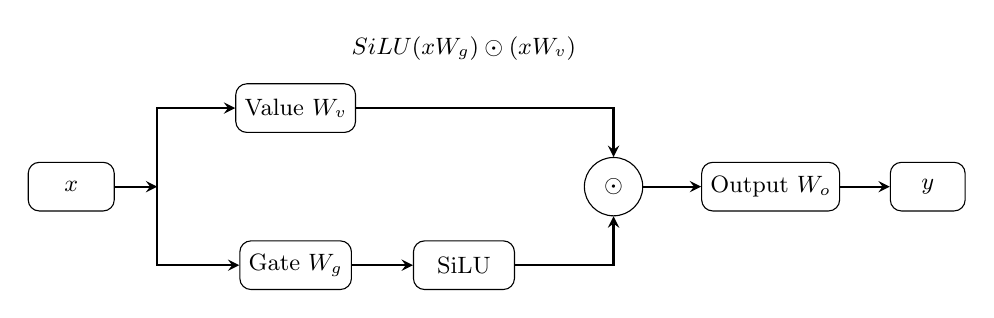
\begin{tikzpicture}[>=stealth, scale=0.95, transform shape, every node/.style={font=\small}]
    \node[draw, rounded corners, minimum width=1.15cm, minimum height=0.65cm]
        (x) at (0,0) {$x$};

    \coordinate (split) at (1.15,0);
    \draw[->, thick] (x) -- (split);

    \node[draw, rounded corners, minimum width=1.45cm, minimum height=0.65cm]
        (wv) at (3.0,1.05) {Value \(W_v\)};
    \node[draw, rounded corners, minimum width=1.45cm, minimum height=0.65cm]
        (wg) at (3.0,-1.05) {Gate \(W_g\)};

    \draw[->, thick] (split) |- (wv.west);
    \draw[->, thick] (split) |- (wg.west);

    \node[draw, rounded corners, minimum width=1.35cm, minimum height=0.65cm]
        (silu) at (5.25,-1.05) {SiLU};
    \draw[->, thick] (wg) -- (silu);

    \node[draw, circle, minimum size=0.78cm] (mul) at (7.25,0)
        {\(\odot\)};
    \draw[->, thick] (wv.east) -| (mul.north);
    \draw[->, thick] (silu.east) -| (mul.south);

    \node[draw, rounded corners, minimum width=1.55cm, minimum height=0.65cm]
        (wo) at (9.35,0) {Output \(W_o\)};
    \node[draw, rounded corners, minimum width=1.0cm, minimum height=0.65cm]
        (y) at (11.45,0) {$y$};
    \draw[->, thick] (mul) -- (wo);
    \draw[->, thick] (wo) -- (y);

    \node at (5.25,1.85)
        {\(\operatorname{SiLU}(xW_g)\odot(xW_v)\)};
\end{tikzpicture}
.
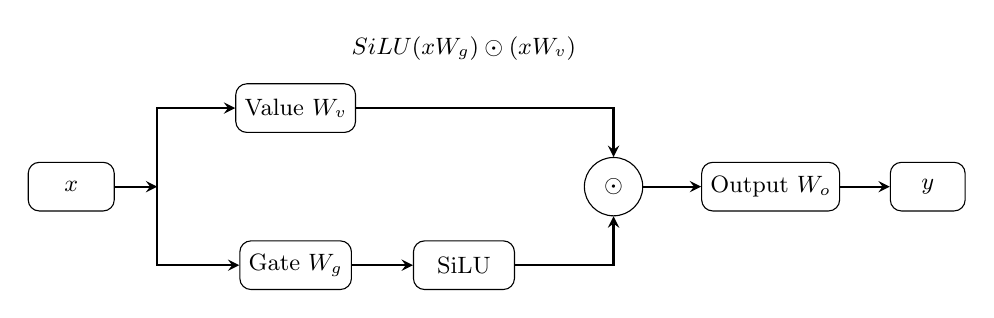
\begin{tikzpicture}[>=stealth, scale=0.95, transform shape, every node/.style={font=\small}]
    \node[draw, rounded corners, minimum width=1.15cm, minimum height=0.65cm]
        (x) at (0,0) {$x$};

    \coordinate (split) at (1.15,0);
    \draw[->, thick] (x) -- (split);

    \node[draw, rounded corners, minimum width=1.45cm, minimum height=0.65cm]
        (wv) at (3.0,1.05) {Value \(W_v\)};
    \node[draw, rounded corners, minimum width=1.45cm, minimum height=0.65cm]
        (wg) at (3.0,-1.05) {Gate \(W_g\)};

    \draw[->, thick] (split) |- (wv.west);
    \draw[->, thick] (split) |- (wg.west);

    \node[draw, rounded corners, minimum width=1.35cm, minimum height=0.65cm]
        (silu) at (5.25,-1.05) {SiLU};
    \draw[->, thick] (wg) -- (silu);

    \node[draw, circle, minimum size=0.78cm] (mul) at (7.25,0)
        {\(\odot\)};
    \draw[->, thick] (wv.east) -| (mul.north);
    \draw[->, thick] (silu.east) -| (mul.south);

    \node[draw, rounded corners, minimum width=1.55cm, minimum height=0.65cm]
        (wo) at (9.35,0) {Output \(W_o\)};
    \node[draw, rounded corners, minimum width=1.0cm, minimum height=0.65cm]
        (y) at (11.45,0) {$y$};
    \draw[->, thick] (mul) -- (wo);
    \draw[->, thick] (wo) -- (y);

    \node at (5.25,1.85)
        {\(\operatorname{SiLU}(xW_g)\odot(xW_v)\)};
\end{tikzpicture}
.
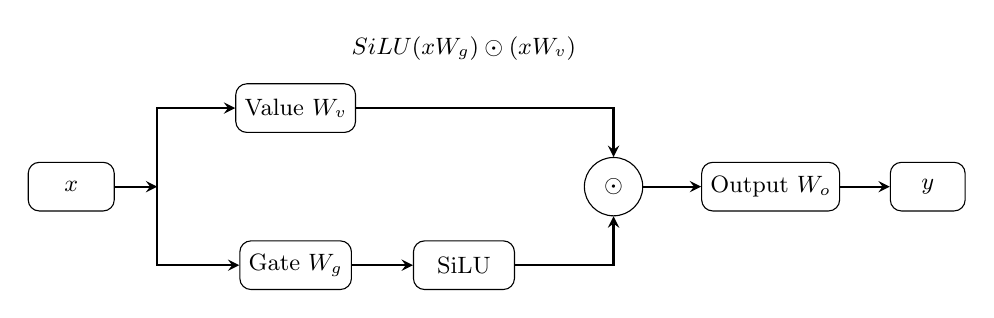
\begin{tikzpicture}[>=stealth, scale=0.95, transform shape, every node/.style={font=\small}]
    \node[draw, rounded corners, minimum width=1.15cm, minimum height=0.65cm]
        (x) at (0,0) {$x$};

    \coordinate (split) at (1.15,0);
    \draw[->, thick] (x) -- (split);

    \node[draw, rounded corners, minimum width=1.45cm, minimum height=0.65cm]
        (wv) at (3.0,1.05) {Value \(W_v\)};
    \node[draw, rounded corners, minimum width=1.45cm, minimum height=0.65cm]
        (wg) at (3.0,-1.05) {Gate \(W_g\)};

    \draw[->, thick] (split) |- (wv.west);
    \draw[->, thick] (split) |- (wg.west);

    \node[draw, rounded corners, minimum width=1.35cm, minimum height=0.65cm]
        (silu) at (5.25,-1.05) {SiLU};
    \draw[->, thick] (wg) -- (silu);

    \node[draw, circle, minimum size=0.78cm] (mul) at (7.25,0)
        {\(\odot\)};
    \draw[->, thick] (wv.east) -| (mul.north);
    \draw[->, thick] (silu.east) -| (mul.south);

    \node[draw, rounded corners, minimum width=1.55cm, minimum height=0.65cm]
        (wo) at (9.35,0) {Output \(W_o\)};
    \node[draw, rounded corners, minimum width=1.0cm, minimum height=0.65cm]
        (y) at (11.45,0) {$y$};
    \draw[->, thick] (mul) -- (wo);
    \draw[->, thick] (wo) -- (y);

    \node at (5.25,1.85)
        {\(\operatorname{SiLU}(xW_g)\odot(xW_v)\)};
\end{tikzpicture}

    \caption{SwiGLU feed-forward computation. The input is mapped through
    parallel value and gate projections. The gate is transformed by SiLU,
    multiplied element-wise by the value representation, and projected
    back to the model hidden dimension. Author-generated schematic based
    on the formulation discussed by \textcite{zhuo2025polycom}.}
    \label{fig:act-swiglu}
\end{figure}
% Alt text for accessibility register: One input branches into a value
% projection and a gate projection. The gate projection passes through
% SiLU. The two branches meet at an element-wise multiplication node,
% followed by an output projection and the output vector.

\subsection{Learnable rational activation functions}
\label{subsec:act-raf}

In a conventional Transformer, the activation function is selected before
pre-training and remains fixed while the weight matrices are optimized.
This separates the choice of activation from the learning process. It
also creates a search problem if different functions may be selected
independently for different layers. If \(k\) candidate functions are
available for each of \(L\) layers, the number of possible layer-wise
configurations is
\begin{equation}
    N_{\mathrm{config}}=k^L.
    \label{eq:act-search-space}
\end{equation}
For \(k=3\) choices and \(L=12\) layers,
\begin{equation}
    N_{\mathrm{config}}=3^{12}=531{,}441.
    \label{eq:act-search-numeric}
\end{equation}
\textcite{fang2023raft} use this example to illustrate why exhaustive
selection of layer-specific activation functions is impractical for
compute-intensive pre-training.

Fang and colleagues investigate rational activation functions (RAFs),
which replace a fixed activation with a rational function whose
coefficients are learned from data. A rational function is a ratio of
polynomials. Their safe parameterization is
\begin{equation}
    F(x)
    =
    \frac{P(x)}{Q_{\mathrm{safe}}(x)}
    =
    \frac{
        \displaystyle\sum_{j=0}^{m}a_jx^j
    }{
        1+
        \left|
            \displaystyle\sum_{k=0}^{n}b_kx^k
        \right|
    },
    \label{eq:act-raf}
\end{equation}
where \(a_j\) and \(b_k\) are trainable coefficients, while \(m\) and
\(n\) are the polynomial degrees. Because
\begin{equation}
    1+
    \left|\sum_{k=0}^{n}b_kx^k\right|
    \geq 1,
    \label{eq:act-raf-denominator-bound}
\end{equation}
the denominator in this parameterization cannot be zero. This is the
stability motivation for the safe rational formulation adopted in
\textcite{fang2023raft}.

The degrees control the flexibility of the rational function. Increasing
them can improve its ability to fit a target activation, but it also
introduces more coefficients and computational work. Fang and colleagues
evaluate degrees in the range \(\{4,5\}\) and select \(m=5\) and \(n=4\)
because this configuration closely fits GELU on the interval
\([-3,3]\). The rational function is presented as a universal function approximator
capable of fitting existing activation profiles. They report nine
additional learnable parameters per implemented rational activation and
108 additional parameters in their 12-layer Transformer, less than \(0.000098\%\) of the original model
parameter count. The paper's reported implementation count is retained
here rather than inferred by counting every coefficient in the generic
displayed expression.

The optimization problem changes when the activation coefficients are
trainable. Let \(\theta\) denote the ordinary Transformer parameters and
let \(\alpha\) collect the rational activation coefficients. Instead of
minimizing only over \(\theta\), training jointly optimizes
\begin{equation}
    (\theta^*,\alpha^*)
    =
    \arg\min_{\theta,\alpha}
    \mathcal{L}(\theta,\alpha;\mathcal{D}),
    \label{eq:act-raf-joint-objective}
\end{equation}
where \(\mathcal{D}\) is the training data and \(\mathcal{L}\) is the
training objective. A gradient-based update can be written as
\begin{align}
    \theta_{t+1}
    &=
    \theta_t-\eta_{\theta}\nabla_{\theta}\mathcal{L},
    \label{eq:act-raf-theta-update}\\
    \alpha_{t+1}
    &=
    \alpha_t-\eta_{\alpha}\nabla_{\alpha}\mathcal{L}.
    \label{eq:act-raf-alpha-update}
\end{align}
The two learning rates need not be equal because the ordinary network
parameters and the activation coefficients can have different
optimization dynamics.

\textcite{fang2023raft} instantiate this approach in a BERT-like
encoder-only Transformer with 12 layers, hidden size 768, and 12
attention heads. They compare a fixed-GELU Transformer (FAFT) with a
rational-activation Transformer (RAFT). Their models are pre-trained
from scratch on English Wikipedia using dynamic masked language
modeling. The paper reports an AdamW configuration with
\(\beta_1=0.9\), \(\beta_2=0.98\), and weight decay \(0.01\). The
learning rate for the ordinary model parameters is \(7\times10^{-4}\),
whereas the learning rate for RAF coefficients is \(5\times10^{-3}\).
Both are warmed up during the first one percent of training steps; the
ordinary parameter learning rate then decays linearly, while the RAF
learning rate remains constant.

The pre-training validation results are
\begin{equation}
    \begin{array}{c|cc}
        \text{Model} & \text{Validation loss} & \text{Perplexity}\\
        \hline
        \text{FAFT} & 1.645 & 5.18\\
        \text{RAFT} & 1.611 & 5.00
    \end{array}
    \label{eq:act-raf-pretraining-results}
\end{equation}
The lower validation loss and perplexity indicate an improvement in
the reported masked-language-modeling evaluation. The authors also
evaluate downstream fine-tuning. With 100 labeled GLUE examples,
RAFT improves the average score over FAFT by 5.31 points when all
model parameters, including RAF coefficients, are fine-tuned
(\(\mathrm{RAFT}_{\mathrm{full}}\)), and by 5.71 points when the
pre-trained RAFs are held fixed
(\(\mathrm{RAFT}_{\mathrm{fixed}}\)). With 300 examples, the reported
average improvements are 0.98 and 1.59 points, respectively. In the
full-data setting, the corresponding improvements are 0.70 and
0.58 points. The paper's abstract reports a 2.05-point improvement
on SQuAD when all available data are used
\parencite{fang2023raft}.

The authors also combine RAFT with BitFit, a parameter-efficient
fine-tuning method that updates bias parameters. In the full-data
setting, the RAFT-based BitFit variants improve over the FAFT-based
BitFit baseline by 2.87 and 3.08 points, depending on whether the
pre-trained RAFs are fixed or fine-tuned. In the low-data setting,
the reported improvements are 3.95 and 4.15 points. The study further
examines fine-tuning only the RAF parameters; it reports 1,178 RAF
parameters in that configuration, while the classification head is
also updated in the experimental setup. These results suggest that
learned activation functions can be useful both as trainable
task-adaptation parameters and as pre-trained transformations that
are subsequently kept fixed.

The learned rational functions differ across Transformer layers after
pre-training. During downstream fine-tuning, the upper layers change more
substantially and develop more task-specific activation profiles than
the lower layers. The authors also report cases in which the output of a
rational activation is close to zero, suggesting that the corresponding
feed-forward branch contributes relatively little to the layer output.
They present the layer- and task-dependent shapes as a possible
additional way to investigate the internal organization of
pre-trained Transformers; similarity between activation profiles,
however, is not by itself proof that two layers encode the same
linguistic properties.

RAF flexibility has a computational cost. In the reported implementation,
training is 36.8\% slower during pre-training and 14.8\% slower during
fine-tuning than the fixed-activation baseline, because the rational
coefficients must also be updated. With their CUDA extension, the
authors report inference speedups of 13.8\% during pre-training
measurements and 3.9\% during fine-tuning measurements. These values
are implementation- and experiment-specific, not hardware-independent
properties of rational functions. The authors also identify limited
training resources as a limitation: their BERT-like experiment is not
a direct comparison with substantially larger publicly available
pre-trained models. They note that the effect of the additional
flexibility on susceptibility to learned data biases requires further
investigation \parencite{fang2023raft}.

\begin{figure}[htbp]
    \centering
    % TikZ source fragment: activation_learnable.tex
% Included by % TikZ source fragment: activation_learnable.tex
% Included by % TikZ source fragment: activation_learnable.tex
% Included by \input{figures/activation_learnable}.
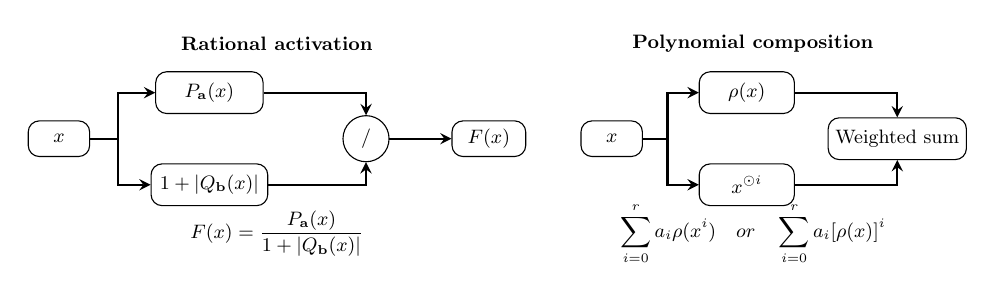
\begin{tikzpicture}[>=stealth, scale=0.78, transform shape, every node/.style={font=\small}]
    % Rational activation panel
    \node[draw, rounded corners, minimum width=1.0cm, minimum height=0.58cm]
        (xr) at (0,0) {$x$};
    \node[draw, rounded corners, minimum width=1.75cm, minimum height=0.68cm]
        (pr) at (2.45,0.75) {\(P_{\mathbf a}(x)\)};
    \node[draw, rounded corners, minimum width=1.9cm, minimum height=0.68cm]
        (qr) at (2.45,-0.75) {\(1+|Q_{\mathbf b}(x)|\)};
    \node[draw, circle, minimum size=0.75cm] (div) at (5.0,0)
        {\(/\)};
    \node[draw, rounded corners, minimum width=1.2cm, minimum height=0.58cm]
        (fr) at (7.0,0) {\(F(x)\)};
    \draw[->, thick] (xr.east) -- ++(0.45,0) |- (pr.west);
    \draw[->, thick] (xr.east) -- ++(0.45,0) |- (qr.west);
    \draw[->, thick] (pr.east) -| (div.north);
    \draw[->, thick] (qr.east) -| (div.south);
    \draw[->, thick] (div) -- (fr);
    \node at (3.55,1.55) {\textbf{Rational activation}};
    \node at (3.55,-1.55)
        {\(\displaystyle F(x)=\frac{P_{\mathbf a}(x)}
        {1+|Q_{\mathbf b}(x)|}\)};

    % Polynomial-composition panel
    \node[draw, rounded corners, minimum width=1.0cm, minimum height=0.58cm]
        (xp) at (9.0,0) {$x$};
    \node[draw, rounded corners, minimum width=1.55cm, minimum height=0.68cm]
        (rho) at (11.2,0.75) {\(\rho(x)\)};
    \node[draw, rounded corners, minimum width=1.55cm, minimum height=0.68cm]
        (pow) at (11.2,-0.75) {\(x^{\odot i}\)};
    \node[draw, rounded corners, minimum width=1.65cm, minimum height=0.68cm]
        (sum) at (13.65,0) {Weighted sum};
    \draw[->, thick] (xp.east) -- ++(0.4,0) |- (rho.west);
    \draw[->, thick] (xp.east) -- ++(0.4,0) |- (pow.west);
    \draw[->, thick] (rho.east) -| (sum.north);
    \draw[->, thick] (pow.east) -| (sum.south);
    \node at (11.3,1.55) {\textbf{Polynomial composition}};
    \node at (11.3,-1.55)
        {\(\displaystyle \sum_{i=0}^{r}a_i\rho(x^i)
        \quad\text{or}\quad
        \sum_{i=0}^{r}a_i[\rho(x)]^i\)};
\end{tikzpicture}
.
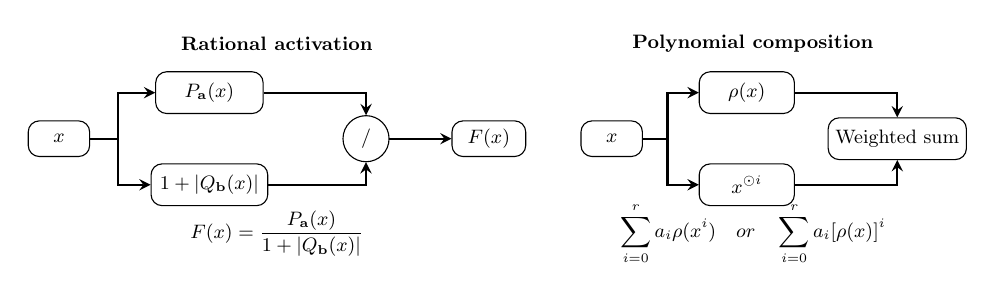
\begin{tikzpicture}[>=stealth, scale=0.78, transform shape, every node/.style={font=\small}]
    % Rational activation panel
    \node[draw, rounded corners, minimum width=1.0cm, minimum height=0.58cm]
        (xr) at (0,0) {$x$};
    \node[draw, rounded corners, minimum width=1.75cm, minimum height=0.68cm]
        (pr) at (2.45,0.75) {\(P_{\mathbf a}(x)\)};
    \node[draw, rounded corners, minimum width=1.9cm, minimum height=0.68cm]
        (qr) at (2.45,-0.75) {\(1+|Q_{\mathbf b}(x)|\)};
    \node[draw, circle, minimum size=0.75cm] (div) at (5.0,0)
        {\(/\)};
    \node[draw, rounded corners, minimum width=1.2cm, minimum height=0.58cm]
        (fr) at (7.0,0) {\(F(x)\)};
    \draw[->, thick] (xr.east) -- ++(0.45,0) |- (pr.west);
    \draw[->, thick] (xr.east) -- ++(0.45,0) |- (qr.west);
    \draw[->, thick] (pr.east) -| (div.north);
    \draw[->, thick] (qr.east) -| (div.south);
    \draw[->, thick] (div) -- (fr);
    \node at (3.55,1.55) {\textbf{Rational activation}};
    \node at (3.55,-1.55)
        {\(\displaystyle F(x)=\frac{P_{\mathbf a}(x)}
        {1+|Q_{\mathbf b}(x)|}\)};

    % Polynomial-composition panel
    \node[draw, rounded corners, minimum width=1.0cm, minimum height=0.58cm]
        (xp) at (9.0,0) {$x$};
    \node[draw, rounded corners, minimum width=1.55cm, minimum height=0.68cm]
        (rho) at (11.2,0.75) {\(\rho(x)\)};
    \node[draw, rounded corners, minimum width=1.55cm, minimum height=0.68cm]
        (pow) at (11.2,-0.75) {\(x^{\odot i}\)};
    \node[draw, rounded corners, minimum width=1.65cm, minimum height=0.68cm]
        (sum) at (13.65,0) {Weighted sum};
    \draw[->, thick] (xp.east) -- ++(0.4,0) |- (rho.west);
    \draw[->, thick] (xp.east) -- ++(0.4,0) |- (pow.west);
    \draw[->, thick] (rho.east) -| (sum.north);
    \draw[->, thick] (pow.east) -| (sum.south);
    \node at (11.3,1.55) {\textbf{Polynomial composition}};
    \node at (11.3,-1.55)
        {\(\displaystyle \sum_{i=0}^{r}a_i\rho(x^i)
        \quad\text{or}\quad
        \sum_{i=0}^{r}a_i[\rho(x)]^i\)};
\end{tikzpicture}
.
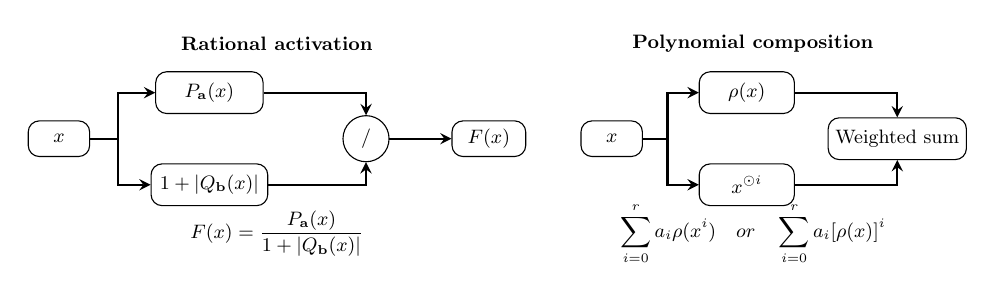
\begin{tikzpicture}[>=stealth, scale=0.78, transform shape, every node/.style={font=\small}]
    % Rational activation panel
    \node[draw, rounded corners, minimum width=1.0cm, minimum height=0.58cm]
        (xr) at (0,0) {$x$};
    \node[draw, rounded corners, minimum width=1.75cm, minimum height=0.68cm]
        (pr) at (2.45,0.75) {\(P_{\mathbf a}(x)\)};
    \node[draw, rounded corners, minimum width=1.9cm, minimum height=0.68cm]
        (qr) at (2.45,-0.75) {\(1+|Q_{\mathbf b}(x)|\)};
    \node[draw, circle, minimum size=0.75cm] (div) at (5.0,0)
        {\(/\)};
    \node[draw, rounded corners, minimum width=1.2cm, minimum height=0.58cm]
        (fr) at (7.0,0) {\(F(x)\)};
    \draw[->, thick] (xr.east) -- ++(0.45,0) |- (pr.west);
    \draw[->, thick] (xr.east) -- ++(0.45,0) |- (qr.west);
    \draw[->, thick] (pr.east) -| (div.north);
    \draw[->, thick] (qr.east) -| (div.south);
    \draw[->, thick] (div) -- (fr);
    \node at (3.55,1.55) {\textbf{Rational activation}};
    \node at (3.55,-1.55)
        {\(\displaystyle F(x)=\frac{P_{\mathbf a}(x)}
        {1+|Q_{\mathbf b}(x)|}\)};

    % Polynomial-composition panel
    \node[draw, rounded corners, minimum width=1.0cm, minimum height=0.58cm]
        (xp) at (9.0,0) {$x$};
    \node[draw, rounded corners, minimum width=1.55cm, minimum height=0.68cm]
        (rho) at (11.2,0.75) {\(\rho(x)\)};
    \node[draw, rounded corners, minimum width=1.55cm, minimum height=0.68cm]
        (pow) at (11.2,-0.75) {\(x^{\odot i}\)};
    \node[draw, rounded corners, minimum width=1.65cm, minimum height=0.68cm]
        (sum) at (13.65,0) {Weighted sum};
    \draw[->, thick] (xp.east) -- ++(0.4,0) |- (rho.west);
    \draw[->, thick] (xp.east) -- ++(0.4,0) |- (pow.west);
    \draw[->, thick] (rho.east) -| (sum.north);
    \draw[->, thick] (pow.east) -| (sum.south);
    \node at (11.3,1.55) {\textbf{Polynomial composition}};
    \node at (11.3,-1.55)
        {\(\displaystyle \sum_{i=0}^{r}a_i\rho(x^i)
        \quad\text{or}\quad
        \sum_{i=0}^{r}a_i[\rho(x)]^i\)};
\end{tikzpicture}

    \caption{Conceptual comparison of rational and polynomial-composition
    activation constructions. A rational activation learns the coefficients
    of a numerator and denominator, whereas PolyCom combines powers and
    another function through learned coefficients. Author-generated
    schematic based on \textcite{fang2023raft} and
    \textcite{zhuo2025polycom}.}
    \label{fig:act-learnable}
\end{figure}
% Alt text for accessibility register: The left panel shows an input
% branching into numerator and denominator polynomial calculations, followed
% by a ratio that produces a rational activation. The right panel shows an
% input transformed through a function and powers, with weighted terms
% combined into a polynomial-composition activation.

\subsection{Polynomial composition activation functions}
\label{subsec:act-polycom}

Learnable rational functions change the coefficients of a rational
approximation during training. A different approach is to construct a
more expressive activation from polynomial terms combined with another
function. \textcite{zhuo2025polycom} introduce Polynomial Composition
Activations (PolyCom) for this purpose. Their motivation is that pure
polynomial activations have limitations in the approximation setting
they discuss and have also shown weak empirical performance in some
deep-learning applications. PolyCom therefore combines polynomial
operations with another function rather than relying on a polynomial
alone.

Let \(\rho\) denote a function such as ReLU, PReLU, sigmoid, SiLU, or
a normalization operation. Let \(r\in\mathbb{N}\) be the polynomial
order and let \(a_i\in\mathbb{R}\) be trainable coefficients. The
authors define two composition types:
\begin{align}
    \operatorname{PolyCom}_{\mathrm{I}}(x)
    &=
    \sum_{i=0}^{r}a_i[\rho(x)]^i,
    \label{eq:act-polycom-type-one}\\
    \operatorname{PolyCom}_{\mathrm{II}}(x)
    &=
    \sum_{i=0}^{r}a_i\rho(x^i).
    \label{eq:act-polycom-type-two}
\end{align}
For vector inputs, powers are applied element-wise. The distinction is
the order of operations. Type I first applies \(\rho\) and then takes
powers of the resulting values. Type II first takes powers of the input
and then applies \(\rho\) to each powered representation. In the
practical experiments, the authors use third-order PolyCom, \(r=3\),
with \(a_0=0\) and \(a_i=1/r\) for \(i=1,\ldots,r\) at initialization;
the coefficients are subsequently trainable.

\paragraph{PolyReLU.}
PolyReLU is a Type I composition in which \(\rho\) is ReLU:
\begin{equation}
    \operatorname{PolyReLU}(x)
    =
    \sum_{i=0}^{r}a_i
    \bigl[\operatorname{ReLU}(x)\bigr]^i,
    \qquad
    \operatorname{ReLU}(x)=\max\{x,0\}.
    \label{eq:act-polyrelu}
\end{equation}
For \(r=3\), the expression is
\begin{equation}
    \operatorname{PolyReLU}(x)
    =
    a_0+a_1\operatorname{ReLU}(x)
    +a_2\operatorname{ReLU}(x)^2
    +a_3\operatorname{ReLU}(x)^3.
    \label{eq:act-polyrelu-cubic}
\end{equation}
For negative inputs, all positive powers of ReLU are zero and the
output is \(a_0\). For positive inputs, the function is a polynomial
in \(x\). The learnable coefficients therefore control the shape of
the positive branch. The paper establishes that ReLU, squared ReLU,
and polynomial activations can be represented as special cases of
PolyReLU \parencite{zhuo2025polycom}.

\paragraph{PolyNorm.}
PolyNorm is a Type II composition in which the powers are normalized
by their Euclidean norms. For a vector
\(x=(x_1,\ldots,x_d)^{\top}\), define its element-wise \(i\)-th power
as
\begin{equation}
    x^{\odot i}
    =
    (x_1^i,\ldots,x_d^i)^{\top}.
    \label{eq:act-elementwise-power}
\end{equation}
The Euclidean norm of a vector \(u\in\mathbb{R}^d\) is
\begin{equation}
    \|u\|_2
    =
    \sqrt{\sum_{j=1}^{d}u_j^2}.
    \label{eq:act-euclidean-norm}
\end{equation}
PolyNorm is then
\begin{equation}
    \operatorname{PolyNorm}(x)
    =
    \sum_{i=0}^{r}
    a_i
    \frac{x^{\odot i}}{\|x^{\odot i}\|_2}.
    \label{eq:act-polynorm}
\end{equation}
Each powered vector is rescaled before the weighted terms are combined.
This is intended to prevent different polynomial orders from having
excessively large or small magnitudes and thereby to stabilize training.
Unlike scalar element-wise activations such as ReLU and GELU, the
normalization denominator depends on the full feature vector. Thus,
each output coordinate of a normalized term depends on the other
coordinates through the common norm. The operation remains local to
the token's feature vector; it does not itself exchange information
between sequence positions. The displayed expression requires a
defined convention if a powered vector has zero norm; the paper's
formula alone does not specify a particular numerical safeguard for
that edge case.

Both PolyReLU and PolyNorm replace the activation in the conventional
feed-forward expression
\begin{equation}
    \operatorname{FFN}_{\rho}(x)=\rho(xW_1)W_2.
    \label{eq:act-polycom-ffn}
\end{equation}
The overall two-projection FFN structure is retained, while the
nonlinear transformation is changed. This differs from SwiGLU, which
adds a parallel projection and a multiplicative gate.

\subsection{Approximation theory and effective dimensionality}
\label{subsec:act-theory}

The theoretical analysis in \textcite{zhuo2025polycom} examines the
expressivity of PolyReLU. A first result is that a ReLU network can
be represented exactly by a PolyReLU network without increasing the
asymptotic network size. Let
\(f:[-1,1]^d\rightarrow[-1,1]\) be a ReLU network with depth \(L\)
and width \(K\). The paper establishes the existence of a PolyReLU
network \(g\) such that
\begin{equation}
    f(x)=g(x)
    \quad\text{for all }x\in[-1,1]^d,
    \qquad
    \operatorname{Size}(g)=O(LK).
    \label{eq:act-polyrelu-exact}
\end{equation}
The construction follows from the fact that ReLU is a special case
of PolyReLU: the corresponding activation in each layer can be
replaced without changing the represented function.

The reverse approximation direction is not equivalent in complexity.
The paper shows that a ReLU network can approximate a fixed-order
PolyReLU activation on a bounded interval with an approximation
error below \(\epsilon\), using a network whose size is
\(O(\log^2(1/\epsilon))\) for the scalar activation approximation.
At the network level, the authors give an upper bound of the form
\begin{equation}
    O\left(
        LK\log^2\left(\frac{L\alpha}{\epsilon}\right)
    \right),
    \label{eq:act-polyrelu-relu-upper}
\end{equation}
under the theorem's assumptions. Here \(L\) is depth, \(K\) is width,
\(\alpha\) is a Lipschitz constant for the PolyReLU activation, and
\(\epsilon\in(0,1)\) is the target uniform approximation tolerance.
A Lipschitz constant bounds how much a function can change when its
input changes:
\begin{equation}
    |\rho(x)-\rho(y)|
    \leq \alpha|x-y|.
    \label{eq:act-lipschitz}
\end{equation}
The authors also establish a lower-bound result of order
\(\Omega(LK\log(1/\epsilon))\) for the corresponding approximation
problem under their stated assumptions. These results concern
function representation and approximation complexity; they do not
by themselves imply that every PolyReLU language model will outperform
every ReLU language model on a particular training distribution.

The paper further studies approximation of smooth functions in
Sobolev spaces. Let \(d\) be the input dimension and let \(s\) denote
the smoothness order. A multi-index
\(\gamma=(\gamma_1,\ldots,\gamma_d)\) has order
\(|\gamma|_1=\sum_{j=1}^{d}\gamma_j\), and
\(D^\gamma f\) denotes the corresponding weak derivative. The
Sobolev space \(W^{s,\infty}([-1,1]^d)\) contains functions whose
weak derivatives through order \(s\) are essentially bounded. A
corresponding norm can be written as
\begin{equation}
    \|f\|_{W^{s,\infty}}
    =
    \max_{|\gamma|_1\leq s}
    \operatorname*{ess\,sup}_{x\in[-1,1]^d}
    |D^\gamma f(x)|.
    \label{eq:act-sobolev-norm}
\end{equation}
The essential supremum is the smallest bound that holds almost
everywhere, allowing exceptions on sets of measure zero. Consider
the unit ball
\begin{equation}
    \mathcal{F}_{s,d}
    =
    \left\{
        f\in W^{s,\infty}([-1,1]^d):
        \|f\|_{W^{s,\infty}}\leq1
    \right\}.
    \label{eq:act-sobolev-ball}
\end{equation}
The paper establishes that, for every \(f\in\mathcal{F}_{s,d}\)
and every \(\epsilon\in(0,1)\), there exists a PolyReLU network
\(g\) such that
\begin{equation}
    \sup_{x\in[-1,1]^d}|f(x)-g(x)|<\epsilon,
    \qquad
    \operatorname{Size}(g)=O(\epsilon^{-d/s}).
    \label{eq:act-polyrelu-sobolev-rate}
\end{equation}
The paper compares this rate with the following reported rates for
other activation families:
\begin{align}
    N_{\mathrm{ReLU}}(\epsilon)
    &=O\left(\epsilon^{-d/s}\log\frac{1}{\epsilon}\right),
    \label{eq:act-relu-sobolev-rate}
    \\
    N_{\mathrm{rational}}(\epsilon)
    &=O\left(\epsilon^{-d/s}\log\log\frac{1}{\epsilon}\right).
    \label{eq:act-rational-sobolev-rate}
\end{align}
Since a corresponding lower bound of order
\(\Omega(\epsilon^{-d/s})\) applies to the function class under
consideration, the PolyReLU rate is optimal in this Sobolev
approximation setting. The conclusion is specific
to the function class, domain, and assumptions of the theorem; it
should not be interpreted as a general theorem about language-model
quality or semantic performance \parencite{zhuo2025polycom}.

The authors also examine the effective rank of feed-forward weight
matrices. Ordinary matrix rank counts the number of nonzero singular
values, but it does not describe how evenly the matrix magnitude is
distributed across singular directions. Let
\begin{equation}
    A=U\Sigma V^{\top}
    \label{eq:act-svd}
\end{equation}
be a singular value decomposition, where the diagonal entries of
\(\Sigma\) are singular values
\(\sigma_1\geq\cdots\geq\sigma_n\geq0\). Define
\begin{equation}
    p_i
    =
    \frac{\sigma_i}{\sum_{j=1}^{n}\sigma_j},
    \qquad i=1,\ldots,n,
    \label{eq:act-singular-probabilities}
\end{equation}
for a nonzero matrix. The values \(p_i\) form a probability
distribution over singular directions. The effective rank is
\begin{equation}
    \operatorname{erank}(A)
    =
    \exp\left(
        -\sum_{i=1}^{n}p_i\ln p_i
    \right),
    \label{eq:act-effective-rank}
\end{equation}
where the convention \(0\ln0=0\) is used. The exponent is the
Shannon entropy of the normalized singular-value distribution.
A more uniform distribution produces a larger effective rank,
whereas concentration in a few singular directions produces a
smaller value. \textcite{zhuo2025polycom} report higher effective
ranks for PolyReLU and PolyNorm FFN weight matrices than for
ReLU, GELU, and SwiGLU in their experiments. This is a structural
observation about the learned matrices, not a direct measure of
semantic understanding.

\subsection{Empirical performance and computational cost}
\label{subsec:act-experiments}

\textcite{zhuo2025polycom} evaluate PolyCom in a dense model and
a Mixture-of-Experts (MoE) model. Their dense model has approximately
1.3 billion parameters, 24 Transformer layers, hidden size 2,048,
and 16 attention heads. It is trained from scratch on RedPajama-1T.
The reported comparison is made after processing 250 billion
training tokens. The MoE model uses the OLMoE framework and has
approximately 6.9 billion total parameters, of which about 1.3
billion are active. It contains 16 layers, hidden size 2,048,
16 attention heads, and 64 experts. The MoE comparison is trained
on 200 billion tokens. The dense experiments use 32 NVIDIA
A100-80G GPUs, and the MoE experiments use 64 such GPUs.

The dense-model results are shown in \cref{tab:act-polycom-dense}.
PolyReLU and PolyNorm achieve lower training loss and validation
perplexity than the compared ReLU, GELU, and SwiGLU configurations.
PolyNorm has the highest average downstream accuracy in the table.
Its average is 1.21 percentage points above SwiGLU in the six
reported downstream tasks. These are results under the paper's
parameter-matched configurations and training setup, not a universal
ranking independent of model size or data.

\begin{table}[htbp]
    \centering
    \caption{Results for the approximately 1.3-billion-parameter dense
    model after 250 billion training tokens. PPL denotes validation
    perplexity; downstream accuracy is averaged across six tasks.
    Source: \textcite{zhuo2025polycom}, Table 1.}
    \label{tab:act-polycom-dense}
    \small
    \begin{tabularx}{\textwidth}{l X c c}
        \toprule
        Activation & Training loss & Validation PPL & Average accuracy \\
        \midrule
        SwiGLU   & 2.19 & 3.22 & 57.47\% \\
        GELU     & 2.20 & 3.24 & 56.98\% \\
        ReLU     & 2.21 & 3.26 & 57.18\% \\
        PolyReLU & 2.17 & 3.18 & 58.22\% \\
        PolyNorm & 2.17 & 3.17 & 58.68\% \\
        \bottomrule
    \end{tabularx}
    \normalsize
\end{table}

For the MoE comparison, the paper evaluates PolyNorm against
SwiGLU. PolyNorm obtains an average validation loss of 2.39,
compared with 2.41 for SwiGLU across the 11 reported validation
datasets. Its average downstream accuracy is 63.37\%, compared
with 62.78\% for SwiGLU across the reported downstream tasks.
PolyNorm outperforms SwiGLU on eight of the ten downstream tasks
reported in the table. Because the MoE experiment compares only
these two activation choices, it does not establish a ranking of
all PolyCom variants against all possible gated activations
\parencite{zhuo2025polycom}.

The polynomial order controls the number of terms in PolyCom.
The ablation study compares second-, third-, and fourth-order
PolyReLU. Increasing the order improves convergence speed in the
reported experiment, but the difference between orders three and
four is not substantial. Higher orders also increase computation
and can create overflow problems, particularly with low-precision
arithmetic. The authors therefore use third-order PolyCom as a
practical compromise. Their composition ablation finds that
PolyNorm gives the lowest training loss among the tested
PolyCom variants, while combining ReLU with normalization does
not improve on PolyNorm. This indicates that additional
compositional complexity is not automatically beneficial.

Activation cost must be compared with that of the feed-forward
matrix operations. For an input tensor
\(X\in\mathbb{R}^{B\times S\times H}\), \textcite{zhuo2025polycom}
use \(24BSH^2\) as the matrix-computation baseline in their
activation-cost analysis and define the ratio
\begin{equation}
    R_{\mathrm{FLOPs}}
    =
    \frac{
        \mathrm{FLOPs}_{\mathrm{activation}}
    }{
        24BSH^2
    }.
    \label{eq:act-flops-ratio}
\end{equation}
This denominator is the source-specific baseline used in their
appendix. It should not be confused with a separate derivation
that counts only two bias-free projection matrix multiplications.

For their illustrative configuration
\(H=1024\), \(B=4\), \(S=4096\), BF16 precision, and third-order
PolyCom, the paper reports the values in
\cref{tab:act-computational-cost}. The ratios are small relative
to the stated matrix-computation baseline, although the
activation-related memory overhead differs across functions.
The values depend on the tensor dimensions, input-scale
assumption, precision, and implementation.

\begin{table}[htbp]
    \centering
    \caption{Activation FLOPs and memory overhead without gradient
    checkpointing for the configuration reported by
    \textcite{zhuo2025polycom}, Table 8.}
    \label{tab:act-computational-cost}
    \small
    \begin{tabularx}{\textwidth}{l X c c}
        \toprule
        Activation & Activation FLOPs & FLOPs ratio & Memory overhead \\
        \midrule
        ReLU     & \(4BSH\)       & \(0.016\%\) & \(128\,\mathrm{MB}\) \\
        GELU     & \(72BSH\)      & \(0.29\%\)  & \(320\,\mathrm{MB}\) \\
        SwiGLU   & \(\frac{112}{3}BSH\) & \(0.15\%\) & \(256\,\mathrm{MB}\) \\
        ReLU\(^{2}\) & \(8BSH\)   & \(0.032\%\) & \(256\,\mathrm{MB}\) \\
        PolyNorm & \(72BSH\)      & \(0.29\%\)  & \(384\,\mathrm{MB}\) \\
        PolyReLU & \(40BSH\)      & \(0.16\%\)  & \(256\,\mathrm{MB}\) \\
        \bottomrule
    \end{tabularx}
    \normalsize
\end{table}

The same appendix reports a separate analysis with gradient
checkpointing. In that setting, the additional activation-memory
overhead is reduced to zero in the table, while activation FLOPs
increase because intermediate values are recomputed during the
backward pass. Checkpointing therefore exchanges computation for
memory. The paper's comparison also adjusts the SwiGLU intermediate
dimension to \(8H/3\) for a parameter-matched comparison with
the \(4H\) intermediate dimension used by the other activations
\parencite{zhuo2025polycom}.

\subsection{Limitations and connection to normalization}
\label{subsec:act-limitations}

The activation functions considered in this section differ in the
architectural components they modify. ReLU, GELU, and SiLU are
scalar nonlinear transformations applied to intermediate features.
GEGLU and SwiGLU use a gating branch and therefore change the
projection structure as well as the nonlinear operation. Rational
activation functions make the activation coefficients trainable,
allowing the shape of the transformation to adapt during training.
PolyCom combines polynomial powers with another function, while
PolyNorm additionally normalizes each powered feature vector.

These approaches involve trade-offs rather than a single universally
optimal choice. ReLU is computationally simple but has zero
derivative on its negative branch. GELU and SiLU provide smooth
alternatives, while gated units add parallel projections and
multiplicative operations. RAFs introduce a small number of
additional parameters in the reported implementation but increase
training computation. PolyCom provides stronger approximation
results under the assumptions studied by its authors and improves
the reported dense- and MoE-model results, but polynomial order
must be controlled to avoid unnecessary computation and numerical
overflow.

The evidence also has scope limitations. The RAF study uses a
BERT-like encoder-only model and explicitly notes its limited
pre-training resources; its results should not be transferred
without qualification to every decoder-only or multimodal
architecture. The PolyCom study covers substantial dense and
MoE training configurations, but its experiments still represent
a finite set of model sizes, datasets, optimization settings,
and evaluation tasks. Neither study establishes that one
activation function dominates in every architecture and
training regime.

The normalization inside PolyNorm should be distinguished from
the normalization sublayers used in Transformer blocks. PolyNorm
normalizes powered feature vectors as part of the activation
construction. Layer normalization and related operations have
a broader architectural role in controlling the statistics and
scale of hidden representations. The activation function and
the normalization sublayer therefore remain conceptually
distinct, even though both can influence numerical stability
and optimization.

The central result of this section is that the activation
function determines a substantial part of the nonlinear
computation performed by the feed-forward network. Its
definition affects the representable mapping, its derivative
affects gradient propagation, and its implementation affects
training cost and numerical stability. Gated, rational, and
polynomial-composition activations extend the design space
beyond a fixed scalar nonlinearity, but their benefits must
be evaluated under explicit architectural and computational
constraints. Having established how intermediate features
are transformed, the next step is to examine normalization
mechanisms, which regulate the scale and statistical
properties of representations as they pass through the
Transformer stack.
